\documentclass[12pt,a4paper]{article}
\usepackage[utf8]{inputenc}
\usepackage[T1]{fontenc}
\usepackage[spanish,es-tabla]{babel}
\usepackage{amsmath,amssymb}
\usepackage{graphicx}
\usepackage{booktabs}
\usepackage{float}
\usepackage[margin=2.5cm]{geometry}
\usepackage{setspace}
\usepackage{hyperref}
\usepackage{algorithm}
\usepackage[noend]{algpseudocode}
\usepackage{caption}
\usepackage{xcolor}
\usepackage{listingsutf8}
\lstset{language=Python,basicstyle=\ttfamily\scriptsize,breaklines=true,frame=single,numbers=left,numberstyle=\tiny,keywordstyle=\bfseries,commentstyle=\itshape\color{gray},showstringspaces=false}
\renewcommand{\lstlistingname}{Código}
\setstretch{1.15}
\hypersetup{colorlinks=true,linkcolor=black,citecolor=blue,urlcolor=blue}


% Corrige el espacio del signo %% en formulas con babel-spanish reciente (Overleaf)
\AtBeginDocument{\DeclareRobustCommand{\%}{\ifmmode\mathchar"0025\else\char37\relax\fi}}
\begin{document}

\begin{titlepage}
\centering
\vspace*{2cm}
{\Large Universidad Autónoma de Bucaramanga (UNAB)\par}
{\large Facultad de Ingeniería -- Ingeniería de Sistemas\par}
\vspace{1cm}
{\large Investigación de Operaciones I\par}
\vspace{2.5cm}
{\LARGE\bfseries Cobertura de clientes con antenas de telefonía:\\[4pt]
formulación Set Cover, solución exacta y Algoritmo Genético\par}
\vspace{2.5cm}
{\large María Isabel Vargas Mendoza\\ Oscar Iván Vera Puerto\par}
\vspace{1.5cm}
{\large Bucaramanga, Colombia\par}
{\large Noviembre de 2026\par}
\end{titlepage}

\tableofcontents
\newpage

\section{Introducción}

El despliegue de una red de telefonía móvil exige decidir en cuáles de un conjunto de ubicaciones candidatas se instalarán antenas para que todos los usuarios queden dentro del área de cobertura de, al menos, una de ellas. Cada ubicación tiene un costo de instalación distinto y cubre a un subconjunto particular de clientes. El objetivo de la empresa es doble: no dejar a ningún cliente sin servicio y hacerlo con el menor costo total posible.

Este problema es una instancia clásica del \textit{problema de cobertura de conjuntos} (\textit{Set Cover Problem}, SCP), uno de los 21 problemas NP-completos de Karp \cite{karp72}. Aparece, además de en telecomunicaciones, en la asignación de personal, la localización de servicios de emergencia, la selección de pruebas de software y el diseño de circuitos. Aunque su enunciado es sencillo, su dificultad computacional crece con el tamaño de la instancia: no se conoce un algoritmo que lo resuelva de forma eficiente en el caso general \cite{garey79}, y resulta difícil incluso de aproximar mejor que un factor logarítmico \cite{feige98}.

En este trabajo se considera una instancia con 500 clientes y 500 ubicaciones candidatas, cuyos subconjuntos de cobertura se entregan en una matriz binaria y cuyos costos se entregan en un archivo aparte. El trabajo plantea el modelo de programación lineal entera binaria del Set Cover y lo resuelve mediante un Algoritmo Genético (AG) diseñado para este problema. Además, para disponer de un punto de referencia, se resuelve el mismo modelo con un solver exacto y se comparan ambos enfoques en calidad de la solución y tiempo de cómputo.

\subsection{Objetivos}
\textbf{Objetivo general.} Determinar el conjunto de antenas de menor costo que cubra a los 500 clientes, modelando el problema como Set Cover y resolviéndolo con un Algoritmo Genético.

\textbf{Objetivos específicos.}
\begin{itemize}
\item Formular el modelo de programación lineal entera binaria del problema, definiendo variables, función objetivo y restricciones.
\item Diseñar e implementar un Algoritmo Genético con operadores de selección, cruce, mutación y reparación adecuados para el Set Cover.
\item Resolver el modelo con un solver exacto y usar su resultado como referencia.
\item Comparar ambos métodos en calidad de solución, tiempo de cómputo y comportamiento, y analizar el efecto de los parámetros del AG.
\end{itemize}

\subsection{Estructura del documento}
La sección 2 presenta el marco teórico. La sección 3 describe la metodología: datos, modelo matemático, método exacto y Algoritmo Genético. La sección 4 reporta y analiza los resultados. La sección 5 presenta las conclusiones.

\section{Marco teórico}

\subsection{El problema de cobertura de conjuntos (Set Cover)}
Sea $U$ un universo de $m$ elementos y sea $\mathcal{S}=\{S_1,\dots,S_n\}$ una colección de subconjuntos de $U$, cada uno con un costo $c_j>0$. El problema de cobertura de conjuntos consiste en elegir una subcolección $\mathcal{C}\subseteq\mathcal{S}$ tal que todo elemento de $U$ pertenezca a al menos un subconjunto elegido, de modo que la suma de los costos de $\mathcal{C}$ sea mínima. Cuando todos los costos son iguales, el problema se reduce a minimizar el número de subconjuntos seleccionados (versión sin pesos); cuando los costos difieren, se habla de la versión ponderada, que es la que se estudia aquí.

En el contexto de telecomunicaciones, el universo $U$ es el conjunto de clientes, cada subconjunto $S_j$ es el conjunto de clientes que quedan cubiertos por una antena instalada en la ubicación $j$, y $c_j$ es el costo de instalar esa antena.

\subsection{Complejidad computacional}
La versión de decisión del Set Cover fue una de las 21 problemas NP-completos identificados por Karp \cite{karp72}. Por tanto, salvo que $\mathrm{P}=\mathrm{NP}$, no existe un algoritmo que lo resuelva en tiempo polinomial para toda instancia \cite{garey79}. Además, Feige \cite{feige98} mostró que, bajo supuestos estándar de complejidad, no es posible aproximarlo con un factor mejor que $(1-\varepsilon)\ln m$. La heurística voraz de Chv\'atal \cite{chvatal79}, que en cada paso elige el subconjunto con menor costo por elemento nuevo cubierto, alcanza una garantía de $H(d)\le 1+\ln d$ veces el óptimo, donde $d$ es el tamaño del subconjunto más grande; esta es esencialmente la mejor garantía posible en el peor caso.

\subsection{Programación lineal entera binaria}
El Set Cover se formula de manera natural como un problema de programación lineal entera binaria (PLEB): las variables de decisión toman únicamente los valores 0 o 1, y tanto la función objetivo como las restricciones son lineales \cite{wolsey98}. La relajación lineal del problema reemplaza la condición $x_j\in\{0,1\}$ por $0\le x_j\le 1$; su valor óptimo es una cota inferior del costo óptimo entero, y es la base de los métodos de solución exacta.

\subsection{Métodos exactos: ramificación y acotamiento}
El método de ramificación y acotamiento (\textit{branch and bound}) \cite{landdoig60} resuelve problemas enteros explorando un árbol de subproblemas. En cada nodo se resuelve la relajación lineal; si su valor es peor que la mejor solución entera conocida (la \textit{incumbente}), el nodo se descarta; si la solución es entera, se actualiza la incumbente; en otro caso se ramifica sobre una variable fraccionaria. Los solvers modernos añaden planos de corte, heurísticas de primal y preprocesamiento. En el caso del Set Cover, Caprara, Fischetti y Toth \cite{caprara00} revisan los algoritmos exactos y heurísticos y muestran que, a medida que crece el número de filas y columnas, los métodos exactos requieren tiempos que pueden volverse prohibitivos aun con solvers de alto desempeño.

\subsection{Metaheurísticas y Algoritmos Genéticos}
Una \textit{metaheurística} es un marco de búsqueda general que no garantiza optimalidad, pero que suele entregar soluciones de buena calidad en tiempos razonables. Los Algoritmos Genéticos, propuestos por Holland \cite{holland75} y popularizados por Goldberg \cite{goldberg89}, se inspiran en la evolución natural. Mantienen una \textit{población} de soluciones candidatas (\textit{cromosomas}) que evoluciona durante varias \textit{generaciones} mediante cuatro mecanismos \cite{eiben15}:
\begin{itemize}
\item \textbf{Evaluación (fitness):} una función que mide la calidad de cada individuo.
\item \textbf{Selección:} los individuos mejores tienen mayor probabilidad de reproducirse; una forma común es la selección por torneo, donde se elige al mejor de $k$ individuos tomados al azar.
\item \textbf{Cruce (\textit{crossover}):} combina el material genético de dos padres para producir hijos; en el cruce uniforme, cada gen del hijo se toma de uno de los dos padres con probabilidad $1/2$.
\item \textbf{Mutación:} modifica aleatoriamente algunos genes para mantener la diversidad y evitar la convergencia prematura.
\end{itemize}
Se suele añadir \textit{elitismo}, que copia los mejores individuos a la siguiente generación sin cambios, de modo que la mejor solución encontrada nunca se pierde.

\subsection{Manejo de restricciones en el Algoritmo Genético}
Un cromosoma binario cualquiera no tiene por qué ser factible: puede dejar clientes sin cubrir. Hay dos estrategias habituales. La primera es \textit{penalizar} el fitness de los individuos infactibles; es simple, pero la población puede pasar mucho tiempo explorando regiones infactibles. La segunda, empleada por Beasley y Chu \cite{beasley96} en su algoritmo genético para el Set Cover, es \textit{reparar} el cromosoma: se agregan columnas hasta lograr factibilidad y luego se eliminan las columnas redundantes. Esta es la estrategia adoptada en este trabajo, pues garantiza que todo individuo evaluado sea una solución válida.

\subsection{Solver utilizado}
Para la solución exacta se usó HiGHS \cite{highs18}, un solver de código abierto para programación lineal y entera mixta, accedido a través de la función \texttt{milp} de SciPy \cite{scipy20}.

\section{Metodología}

\subsection{Descripción de los datos}
Se dispone de dos archivos. El primero, \texttt{set\_cover\_500x500.csv}, es una matriz de $500\times 500$ con valores 0 y 1, donde la entrada de la fila $i$ y la columna $j$ vale 1 si la antena ubicada en $j$ cubre al cliente $i$. El segundo, \texttt{Costo\_S.xlsx}, contiene el costo de instalación de cada una de las 500 antenas.

La matriz tiene una densidad de 0,0999, es decir, cerca del 10\,\% de las entradas son unos. Cada cliente queda cubierto por entre 32 y 70 antenas, y cada antena cubre entre 33 y 66 clientes. Los costos van de 2\,000 a 3\,998, con un promedio de 3\,033,6. La Figura~\ref{fig:datos} muestra la distribución de los costos y de la cobertura por cliente. Como todo cliente tiene al menos 32 antenas que lo cubren, la instancia es factible (por ejemplo, instalando todas las antenas).

\begin{figure}[H]
\centering
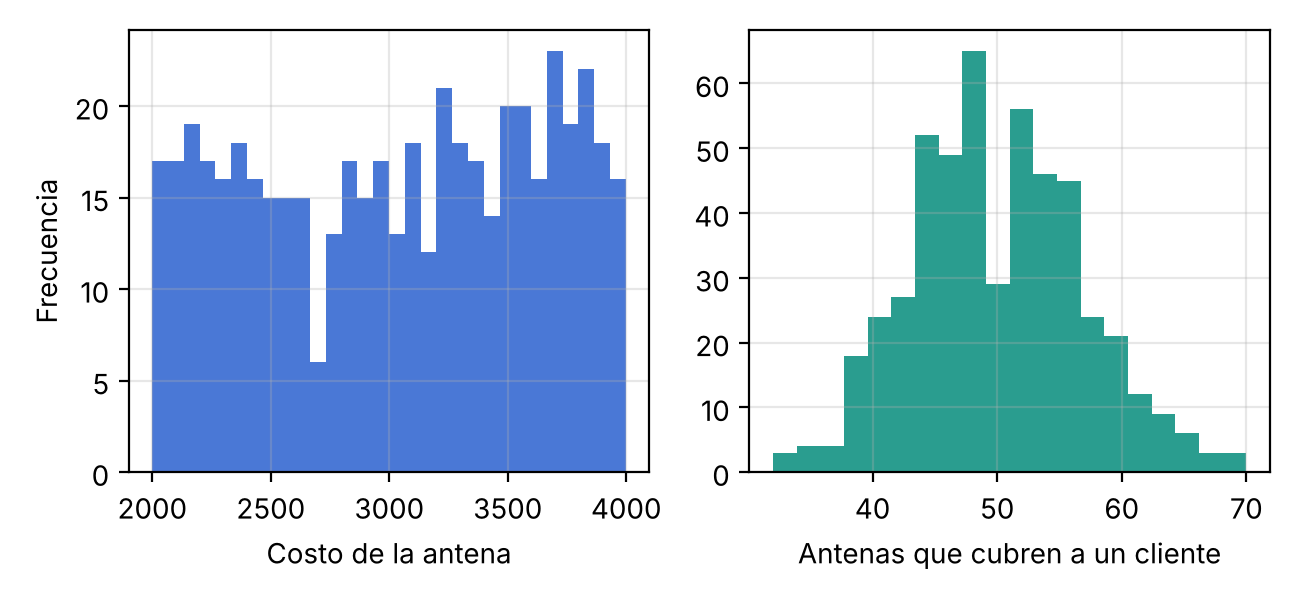
\includegraphics[width=0.85\textwidth]{figuras/datos.png}
\caption{Distribución de los costos de las antenas y del número de antenas que cubren a cada cliente.}
\label{fig:datos}
\end{figure}

\subsection{Formulación matemática}

\paragraph{Conjuntos e índices.}
$I=\{1,\dots,500\}$ es el conjunto de clientes, indexado por $i$; $J=\{1,\dots,500\}$ es el conjunto de ubicaciones de antenas, indexado por $j$.

\paragraph{Parámetros.}
\begin{itemize}
\item $a_{ij}\in\{0,1\}$: vale 1 si la antena $j$ cubre al cliente $i$ y 0 en caso contrario.
\item $c_j>0$: costo de instalar la antena $j$.
\end{itemize}

\paragraph{Variables de decisión.}
\[
x_j=\begin{cases}1 & \text{si se instala una antena en la ubicación } j,\\ 0 & \text{en caso contrario,}\end{cases}\qquad j\in J.
\]

\paragraph{Modelo.}
\begin{align}
\min\; Z &= \sum_{j\in J} c_j\,x_j \label{eq:obj}\\
\text{s.a.}\quad \sum_{j\in J} a_{ij}\,x_j &\ge 1 \qquad \forall\, i\in I \label{eq:cob}\\
x_j &\in\{0,1\} \qquad \forall\, j\in J \label{eq:bin}
\end{align}

\paragraph{Significado de cada componente.}
La función objetivo \eqref{eq:obj} es el costo total de las antenas instaladas, que se desea minimizar. Las restricciones \eqref{eq:cob} garantizan la cobertura: para cada cliente $i$, la suma $\sum_j a_{ij}x_j$ cuenta cuántas antenas instaladas lo cubren, y debe ser al menos 1. Las restricciones \eqref{eq:bin} indican que cada ubicación se usa o no se usa; no se pueden instalar fracciones de antena. El modelo tiene 500 variables binarias y 500 restricciones de cobertura.

\subsection{Solución exacta}
El modelo \eqref{eq:obj}--\eqref{eq:bin} se implementó en Python y se resolvió con el solver HiGHS \cite{highs18} mediante la función \texttt{scipy.optimize.milp}. Se fijó un límite de tiempo de 600 segundos y una brecha relativa de optimalidad de 0. Se registraron el costo de la mejor solución entera, la cota inferior del solver, la brecha entre ambos y el tiempo de cómputo.

\subsection{Algoritmo Genético}

\paragraph{Codificación.}
Cada individuo es un vector binario $\mathbf{x}=(x_1,\dots,x_{500})$ con la misma interpretación que las variables del modelo: $x_j=1$ si se instala la antena $j$.

\paragraph{Reparación.}
Dado un vector $\mathbf{x}$ cualquiera, se aplica el procedimiento de reparación de dos fases, inspirado en Beasley y Chu \cite{beasley96}:
\begin{enumerate}
\item \textbf{Fase de cobertura:} mientras haya clientes sin cubrir, se agrega la antena que minimiza la razón $c_j / n_j$, donde $n_j$ es el número de clientes sin cubrir que la antena $j$ cubriría. Esto es el criterio voraz de Chv\'atal \cite{chvatal79}.
\item \textbf{Fase de eliminación de redundancias:} se recorren las antenas instaladas de la más cara a la más barata y se elimina cada una cuya salida deje a todos sus clientes con al menos otra antena.
\end{enumerate}

\paragraph{Fitness.}
Como todo individuo reparado es factible, el fitness es simplemente el costo $f(\mathbf{x})=\sum_j c_jx_j$, que se minimiza.

\paragraph{Inicialización.}
Cada individuo de la población inicial se genera activando cada gen con probabilidad $p_{\text{init}}=0{,}05$ y reparando el resultado. Esto produce individuos diversos y factibles desde el comienzo.

\paragraph{Selección.}
Se usa selección por torneo de tamaño $k=3$: se toman $k$ individuos al azar y se elige el de menor costo.

\paragraph{Cruce.}
Con probabilidad $p_c=0{,}9$, los dos padres se combinan mediante cruce uniforme: cada gen del hijo se toma de un padre u otro con probabilidad $1/2$. Con probabilidad $1-p_c$ el hijo es copia del primer padre.

\paragraph{Mutación.}
Cada gen del hijo se invierte de forma independiente con probabilidad $p_m=1/n=0{,}002$, de modo que en promedio se muta un gen por hijo. Tras la mutación el hijo se repara.

\paragraph{Elitismo y criterio de parada.}
Los 2 mejores individuos pasan sin cambios a la siguiente generación. El algoritmo se detiene al llegar a 300 generaciones o cuando el mejor costo no mejora durante 80 generaciones consecutivas.

\paragraph{Parámetros.}
La Tabla~\ref{tab:params} resume los parámetros de la configuración base y las variantes que se estudiaron.

\begin{table}[H]
\centering
\caption{Parámetros del Algoritmo Genético.}
\label{tab:params}
\begin{tabular}{lcccc}
\toprule
Parámetro & Base & Población pequeña & Población grande & Mutación alta\\
\midrule
Tamaño de población & 100 & 30 & 300 & 100\\
Probabilidad de cruce & 0,9 & 0,9 & 0,9 & 0,9\\
Probabilidad de mutación por gen & $1/500$ & $1/500$ & $1/500$ & $5/500$\\
Tamaño del torneo & 3 & 3 & 3 & 3\\
Élite & 2 & 2 & 2 & 2\\
Máx. generaciones & 300 & 300 & 300 & 300\\
Paciencia (generaciones) & 80 & 80 & 80 & 80\\
\bottomrule
\end{tabular}
\end{table}

\begin{algorithm}[H]
\caption{Algoritmo Genético con reparación para el Set Cover}
\begin{algorithmic}[1]
\State Generar población inicial de $N$ individuos y repararlos
\State Evaluar el costo de cada individuo
\For{$g=1,\dots,G_{\max}$}
  \State Copiar los $E$ mejores individuos a la nueva población (elitismo)
  \While{la nueva población tenga menos de $N$ individuos}
    \State Seleccionar dos padres por torneo
    \State Con probabilidad $p_c$ aplicar cruce uniforme; si no, copiar el primer padre
    \State Mutar cada gen con probabilidad $p_m$
    \State Reparar el hijo y agregarlo a la nueva población
  \EndWhile
  \State Evaluar la nueva población y actualizar la mejor solución
  \If{no hubo mejora en $P$ generaciones} \State \textbf{parar} \EndIf
\EndFor
\State \Return mejor solución encontrada
\end{algorithmic}
\end{algorithm}

\subsection{Diseño experimental}
Los algoritmos se implementaron en Python con NumPy y SciPy \cite{scipy20}. El AG es estocástico, por lo que un único resultado no es representativo: cada configuración de la Tabla~\ref{tab:params} se ejecutó 10 veces con semillas distintas (0 a 9). Se registraron el costo final, el número de antenas, el número de generaciones y el tiempo de cómputo. Además se ejecutó una configuración \textit{extendida} (población de 200, mutación $2/n$, hasta 3\,000 generaciones y paciencia de 400) con otras 10 semillas, para estudiar el efecto de una búsqueda más larga. Como referencias adicionales se calcularon la heurística voraz de Chv\'atal y la cota inferior de la relajación lineal. Para comparar con el método exacto se calculó la brecha relativa
\[
\text{Brecha}=\frac{Z_{\text{AG}}-Z_{\text{ref}}}{Z_{\text{ref}}}\times 100\,\%,
\]
donde $Z_{\text{ref}}$ es el costo de la mejor solución entera del solver exacto.

\subsection{Interfaz visual}
Se desarrolló una aplicación web con Streamlit que permite cargar los datos, ejecutar el solver exacto y el AG con parámetros ajustables, ver las curvas de convergencia y comparar ambos métodos en costo, tiempo y antenas seleccionadas.

\section{Resultados}

\subsection{Entorno de ejecución}
Los algoritmos se implementaron en Python con NumPy y SciPy \cite{scipy20}. El solver exacto es HiGHS \cite{highs18} con un límite de tiempo de 600 segundos. El Algoritmo Genético se ejecutó con semillas distintas para cada corrida. Los tiempos de cómputo dependen del equipo en que se ejecuta el código, por lo que deben leerse como una comparación relativa entre métodos y no como valores absolutos.

\subsection{Solución exacta}
El solver HiGHS no logró demostrar la optimalidad en los 600 segundos permitidos. Terminó con la mejor solución entera encontrada, de \textbf{costo 50\,119} y 22 antenas, una cota inferior (\textit{dual bound}) de 30\,817 y una brecha de optimalidad de 38,5\,\%. Exploró 19\,036 nodos del árbol de ramificación. La relajación lineal del modelo, que se resuelve en menos de un segundo, da una cota inferior de 27\,860. Es decir, el costo óptimo está entre 30\,817 y 50\,119, según lo que el solver pudo demostrar.

Este comportamiento es el esperado para una instancia densa de $500\times500$: cada cliente tiene entre 32 y 70 antenas que lo cubren, de modo que hay muchísimas combinaciones casi equivalentes y la cota inferior mejora muy lentamente, como lo discuten Caprara, Fischetti y Toth \cite{caprara00}.

\subsection{Heurística voraz de referencia}
Como referencia adicional se aplicó la heurística voraz de Chv\'atal \cite{chvatal79}, que es la fase de cobertura de la reparación del Algoritmo Genético. Obtuvo un costo de 52\,063 con 23 antenas en menos de 0,01 segundos.

\subsection{Algoritmo Genético}
La Tabla~\ref{tab:ga} resume 10 corridas independientes por configuración. La configuración \textit{extendida} usa población de 200, mutación $2/n$, hasta 3\,000 generaciones y paciencia de 400 generaciones.

\begin{table}[H]
\centering
\caption{Resultados del Algoritmo Genético (10 corridas por configuración). La brecha se mide contra la mejor solución entera del solver exacto (50\,119); un valor negativo significa que el AG obtuvo menor costo.}
\label{tab:ga}
\small
\begin{tabular}{lrrrrrrr}
\toprule
Configuración & Mejor & Media & Desv. & Peor & Tiempo (s) & Brecha mejor & Brecha media\\
\midrule
Base ($N=100$, $p_m=1/n$) & 48\,878 & 51\,622 & 1\,500 & 53\,807 & 2,1 & $-2{,}5\,\%$ & $+3{,}0\,\%$\\
Población pequeña ($N=30$) & 50\,914 & 54\,134 & 1\,712 & 57\,351 & 0,7 & $+1{,}6\,\%$ & $+8{,}0\,\%$\\
Población grande ($N=300$) & 49\,774 & 50\,809 & 992 & 53\,414 & 7,3 & $-0{,}7\,\%$ & $+1{,}4\,\%$\\
Mutación alta ($p_m=5/n$) & 49\,678 & 51\,452 & 1\,328 & 53\,976 & 3,1 & $-0{,}9\,\%$ & $+2{,}7\,\%$\\
Extendida ($N=200$, $p_m=2/n$) & 49\,678 & 50\,436 & 606 & 52\,038 & 16,6 & $-0{,}9\,\%$ & $+0{,}6\,\%$\\
\bottomrule
\end{tabular}
\end{table}

\begin{figure}[H]
\centering
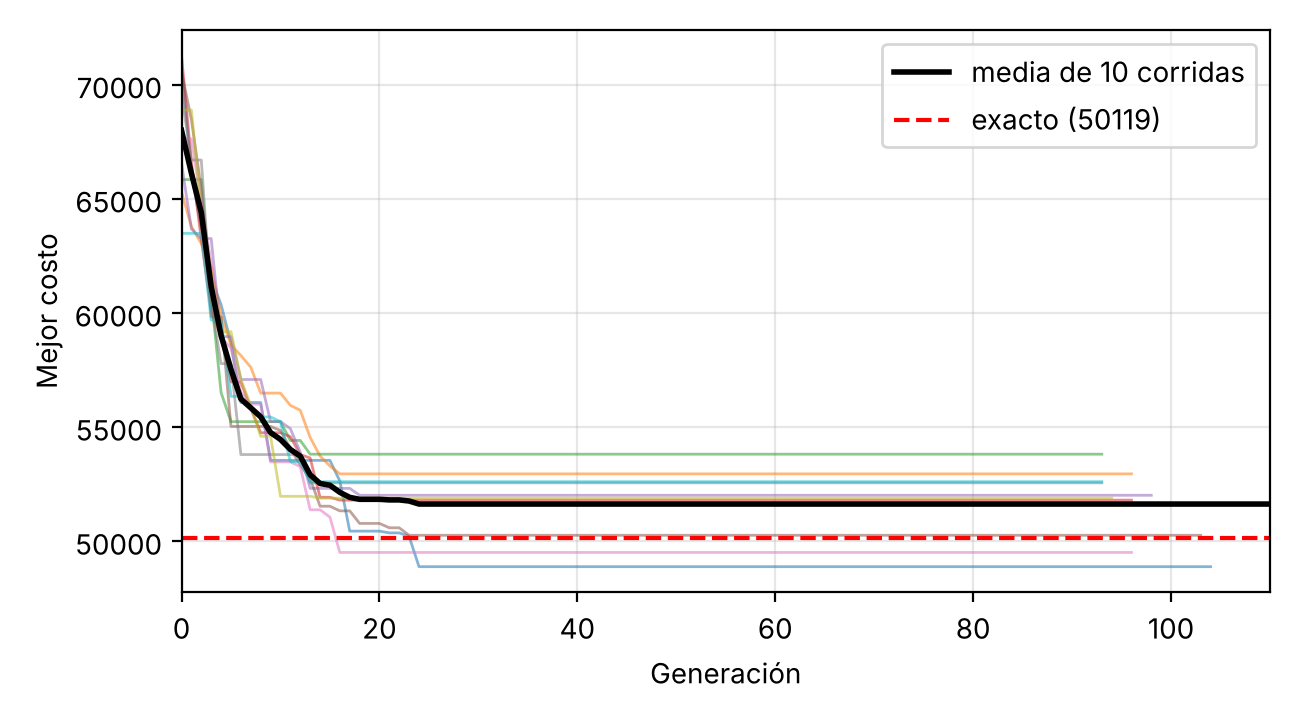
\includegraphics[width=0.85\textwidth]{figuras/convergencia.png}
\caption{Convergencia del Algoritmo Genético (configuración base). Las líneas delgadas son las 10 corridas; la línea gruesa es su promedio; la línea roja punteada es el costo de la mejor solución del solver exacto.}
\label{fig:conv}
\end{figure}

La Figura~\ref{fig:conv} muestra que el AG mejora rápidamente en las primeras 20 a 25 generaciones, partiendo de costos cercanos a 68\,000, y después se estanca: la mayoría de las corridas deja de mejorar y se detiene por el criterio de paciencia hacia la generación 100. Esto indica convergencia prematura: la población pierde diversidad y el cruce deja de producir mejoras.

\begin{figure}[H]
\centering
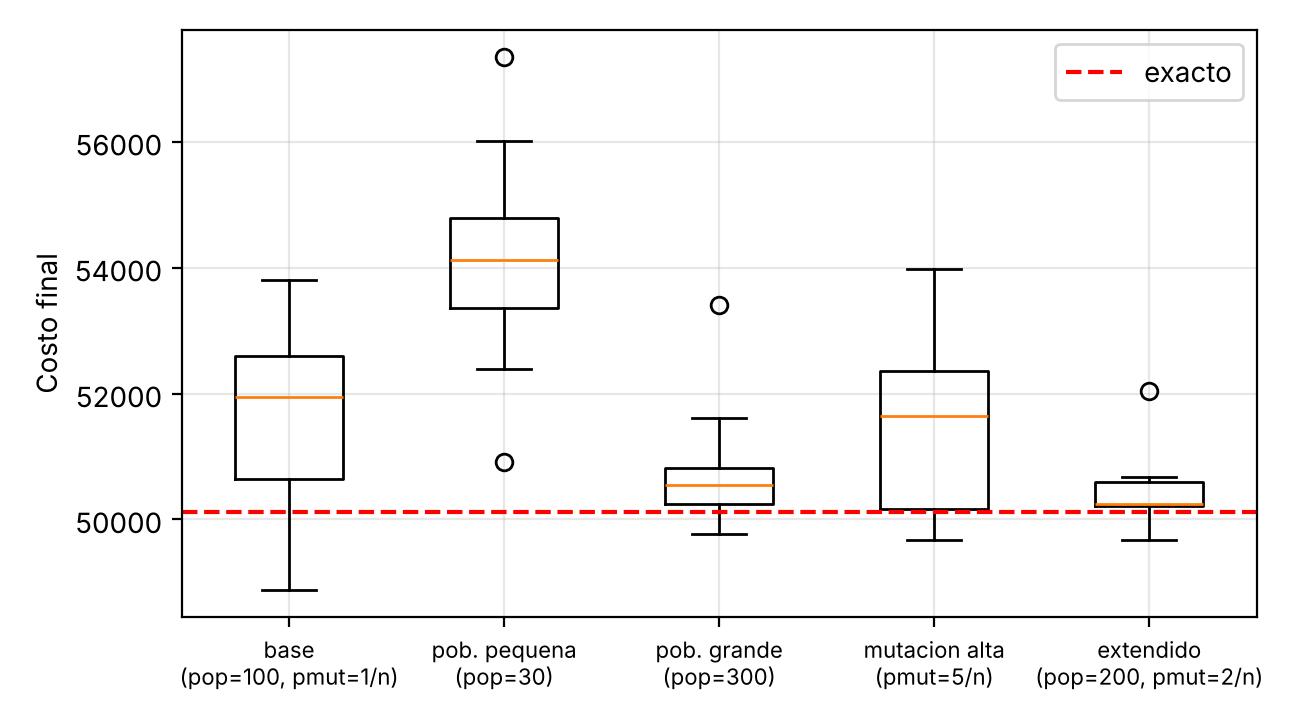
\includegraphics[width=0.85\textwidth]{figuras/boxplot_config.png}
\caption{Distribución del costo final por configuración del AG (10 corridas cada una). La línea roja es la mejor solución del solver exacto.}
\label{fig:box}
\end{figure}

\subsection{Comparación entre el método exacto y el Algoritmo Genético}
La Figura~\ref{fig:comp} compara los costos de todos los métodos y la Tabla~\ref{tab:comp} los resume junto con sus tiempos.

\begin{figure}[H]
\centering
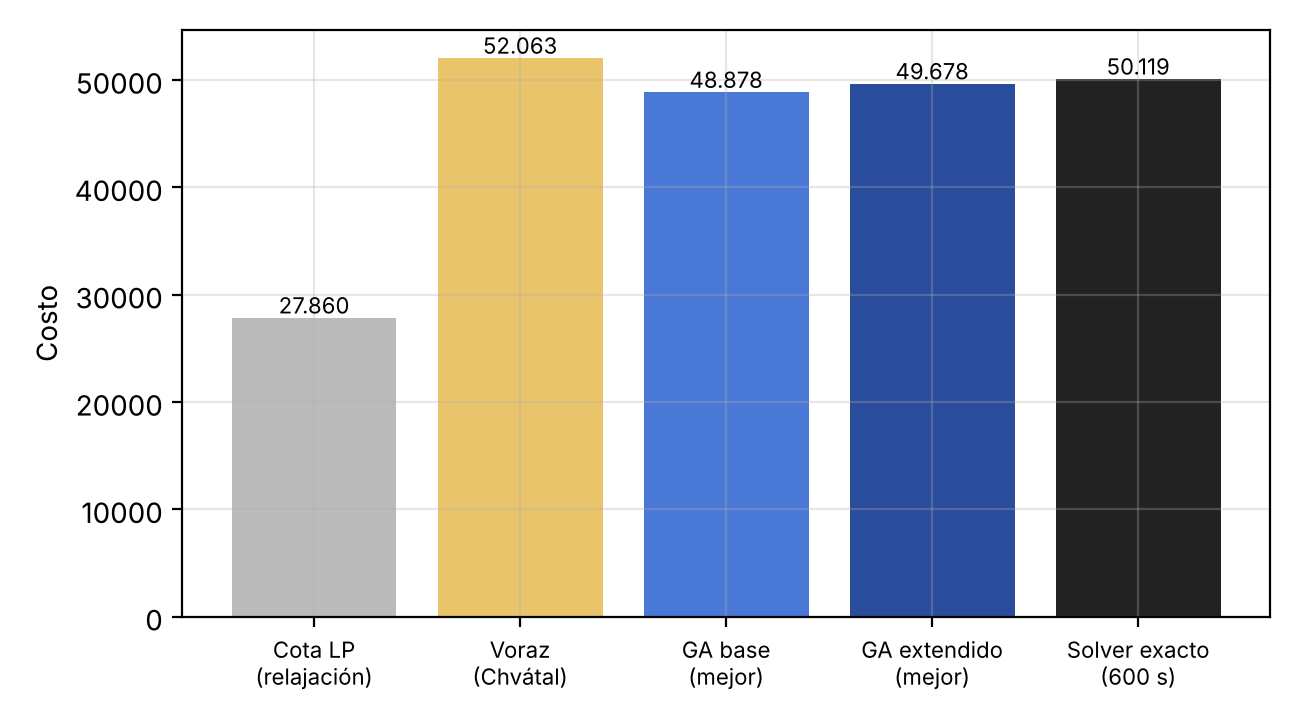
\includegraphics[width=0.85\textwidth]{figuras/comparacion.png}
\caption{Costo obtenido por cada método.}
\label{fig:comp}
\end{figure}

\begin{table}[H]
\centering
\caption{Comparación de métodos.}
\label{tab:comp}
\begin{tabular}{lrrr}
\toprule
Método & Costo & Antenas & Tiempo (s)\\
\midrule
Cota inferior (relajación lineal) & 27\,860 & -- & 0,2\\
Cota inferior del solver (600 s) & 30\,817 & -- & 600\\
Solver exacto (mejor entera) & 50\,119 & 22 & 600\\
Heurística voraz & 52\,063 & 23 & $<0{,}01$\\
AG base (mejor de 10) & 48\,878 & -- & 2,1 (promedio)\\
AG base (media de 10) & 51\,622 & 23,6 & 2,1\\
AG extendido (media de 10) & 50\,436 & 23,0 & 16,6\\
\bottomrule
\end{tabular}
\end{table}

\begin{figure}[H]
\centering
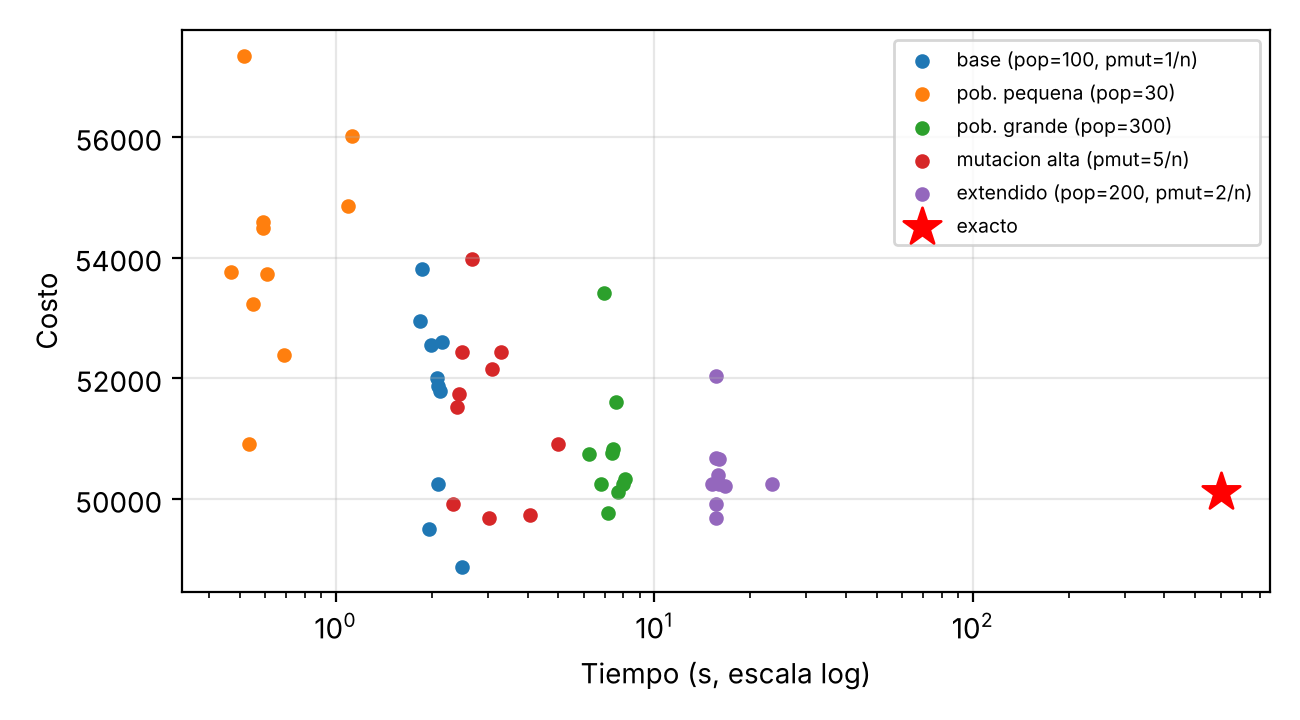
\includegraphics[width=0.85\textwidth]{figuras/costo_vs_tiempo.png}
\caption{Costo frente al tiempo de cómputo (escala logarítmica en el tiempo). La estrella roja es el solver exacto.}
\label{fig:tiempo}
\end{figure}

\subsection{Análisis}
\textbf{Calidad de la solución.} La mejor solución encontrada por el AG (48\,878, en la configuración base) es 2,5\,\% más barata que la mejor solución entera que el solver encontró en 600 segundos, y 6,1\,\% más barata que la heurística voraz. Sin embargo, el AG es estocástico: en la configuración base el costo medio es 3,0\,\% mayor que el del solver y varía entre 48\,878 y 53\,807. La configuración extendida es más estable (desviación de 606) y su media queda a 0,6\,\% del solver.

\textbf{Tiempo de cómputo.} El AG base necesita unos 2 segundos por corrida; el solver agotó 600 segundos sin demostrar optimalidad. El AG llega a soluciones de calidad comparable en una fracción del tiempo.

\textbf{Efecto de los parámetros.} Una población pequeña ($N=30$) empeora claramente los resultados (media $+8{,}0\,\%$ sobre el solver) porque explora poco. Una población mayor reduce la media y la dispersión, pero cuesta más tiempo (7,3\,s con $N=300$). Aumentar la mutación a $5/n$ mejora levemente el mejor resultado sin costo de tiempo importante. La configuración extendida logra la mejor media y la menor dispersión al precio de unos 17 segundos.

\textbf{¿El AG alcanzó el óptimo?} No se puede afirmar. El solver no demostró la optimalidad, y su mejor cota inferior es 30\,817, de modo que el costo óptimo está entre 30\,817 y 48\,878 (la mejor solución conocida). Lo que sí se puede afirmar es que el AG obtuvo soluciones factibles de menor costo que las del solver en el tiempo límite. Para saber qué tan lejos está del óptimo haría falta un solver con más tiempo o una cota inferior más fuerte.

\section{Conclusiones}

\begin{enumerate}
\item El problema de cobertura de antenas se formuló como un modelo de programación lineal entera binaria con 500 variables y 500 restricciones de cobertura, que minimiza el costo total de instalación y exige que cada cliente sea cubierto por al menos una antena.
\item Para esta instancia densa de $500\times500$, el solver exacto HiGHS no logró demostrar la optimalidad en 600 segundos: terminó con una solución de costo 50\,119 y una brecha de 38,5\,\% respecto a su mejor cota inferior. Esto ilustra por qué el Set Cover, por ser NP-difícil, es costoso de resolver de forma exacta cuando crece el tamaño de la instancia.
\item El Algoritmo Genético con reparación diseñado encontró soluciones factibles en pocos segundos. Su mejor resultado (48\,878) fue 2,5\,\% más barato que la mejor solución del solver en el tiempo límite, y 6,1\,\% más barato que la heurística voraz. El AG es entonces una alternativa práctica cuando el tiempo de cómputo es limitado.
\item El AG es estocástico: el costo varía de una corrida a otra (desviación de unos 1\,500 en la configuración base). Aumentar la población o usar una búsqueda más larga reduce esa variabilidad (desviación de 606 en la configuración extendida), a cambio de más tiempo.
\item El AG mostró convergencia prematura: mejora rápido en las primeras generaciones y luego se estanca. Estrategias como mayor mutación, mecanismos de diversidad o búsqueda local podrían mejorar los resultados.
\item No es posible afirmar que el AG alcanzó el óptimo, porque el solver no lo demostró. El óptimo está entre 30\,817 y 48\,878.
\end{enumerate}

\subsection*{Limitaciones y trabajo futuro}
El estudio usa una sola instancia, un solo solver y un límite de 600 segundos. Trabajo futuro: dar más tiempo al solver o usar la solución del AG como punto de partida del método exacto, probar otros operadores de cruce y de selección, incorporar búsqueda local, y evaluar el método en más instancias, por ejemplo las de la OR-Library, con pruebas estadísticas entre configuraciones.


\appendix
\section*{Anexos y apéndices}
\addcontentsline{toc}{section}{Anexos y apéndices}
\renewcommand{\thesubsection}{\Alph{subsection}}
En el \textbf{Anexo} se describe el material entregado por el docente (los datos de la instancia). Los \textbf{Apéndices} contienen material elaborado por los autores: resultados completos, la solución exacta, el código fuente y las instrucciones para reproducir todo.

\subsection*{Anexo A. Instancia entregada por el docente}
\addcontentsline{toc}{subsection}{Anexo A. Instancia entregada por el docente}

La instancia consiste en una matriz binaria $A$ de 500$\times$500 (filas: clientes; columnas: antenas), donde $a_{ij}=1$ si la antena $j$ cubre al cliente $i$, y un vector de costos $c_j$ por antena. La Tabla~\ref{tab:instancia} resume sus características.
\begin{table}[H]
\centering
\caption{Características de la instancia}
\label{tab:instancia}
\begin{tabular}{lr}
\toprule
Característica & Valor \\
\midrule
Clientes (restricciones) & 500 \\
Antenas (variables) & 500 \\
Densidad de la matriz (proporción de unos) & 0.100 \\
Antenas que cubren a cada cliente (mín. / media / máx.) & 32 / 49.9 / 70 \\
Clientes que cubre cada antena (mín. / media / máx.) & 33 / 49.9 / 66 \\
Costo por antena (mín. / media / máx.) & 2\,000 / 3\,034 / 3\,998 \\
Costo de instalar todas las antenas & 1\,516\,821 \\
\bottomrule
\end{tabular}
\end{table}

\subsection*{Apéndice A. Resultados del Algoritmo Genético por corrida}
\addcontentsline{toc}{subsection}{Apéndice A. Resultados del Algoritmo Genético por corrida}

\begin{table}[H]
\centering
\caption{Configuración base (población 100, mutación $1/n$): resultado de cada corrida}
\label{tab:ap_base}
\begin{tabular}{rrrrr}
\toprule
Semilla & Costo & Antenas & Generaciones & Tiempo (s) \\
\midrule
0 & 48\,878 & 22 & 104 & 2.5 \\
1 & 52\,945 & 25 & 96 & 1.8 \\
2 & 53\,807 & 24 & 93 & 1.9 \\
3 & 51\,793 & 24 & 96 & 2.1 \\
4 & 52\,007 & 24 & 98 & 2.1 \\
5 & 50\,253 & 23 & 103 & 2.1 \\
6 & 49\,501 & 22 & 96 & 2.0 \\
7 & 52\,551 & 24 & 93 & 2.0 \\
8 & 51\,881 & 24 & 94 & 2.1 \\
9 & 52\,603 & 24 & 93 & 2.2 \\
\midrule
Mejor / media / peor & \multicolumn{4}{r}{48\,878 / 51\,622 / 53\,807} \\
\bottomrule
\end{tabular}
\end{table}
\begin{table}[H]
\centering
\caption{Configuración extendida (población 200, mutación $2/n$): resultado de cada corrida}
\label{tab:ap_ext}
\begin{tabular}{rrrrr}
\toprule
Semilla & Costo & Antenas & Generaciones & Tiempo (s) \\
\midrule
100 & 50\,209 & 22 & 449 & 16.6 \\
101 & 50\,253 & 23 & 617 & 23.5 \\
102 & 50\,403 & 23 & 423 & 15.8 \\
103 & 50\,681 & 23 & 421 & 15.7 \\
104 & 50\,669 & 23 & 425 & 16.0 \\
105 & 50\,253 & 23 & 416 & 15.2 \\
106 & 49\,678 & 23 & 418 & 15.6 \\
107 & 50\,253 & 23 & 419 & 16.0 \\
108 & 49\,920 & 23 & 421 & 15.6 \\
109 & 52\,038 & 24 & 415 & 15.7 \\
\midrule
Mejor / media / peor & \multicolumn{4}{r}{49\,678 / 50\,436 / 52\,038} \\
\bottomrule
\end{tabular}
\end{table}

\subsection*{Apéndice B. Mejor solución entera del método exacto}
\addcontentsline{toc}{subsection}{Apéndice B. Mejor solución entera del método exacto}
HiGHS terminó por límite de tiempo (600 s), por lo que esta solución es la mejor encontrada y no está certificada como óptima: costo 50\,119, cota inferior 30\,817 y brecha 38.51\,\%. Las 22 antenas seleccionadas (numeradas desde 1) son:

\begin{quote}
13, 19, 44, 45, 73, 79, 94, 200, 210, 277, 307, 334, 357, 366, 401, 404, 411, 432, 444, 450, 473, 475.
\end{quote}

\subsection*{Apéndice C. Código fuente}
\addcontentsline{toc}{subsection}{Apéndice C. Código fuente}
Se incluyen los tres módulos centrales. El código completo (experimentos, figuras e interfaz) está en el repositorio indicado en el Apéndice D.

\lstinputlisting[caption={Carga de datos (\texttt{setcover\_datos.py})}]{codigo/setcover_datos.py}
\lstinputlisting[caption={Solución exacta con HiGHS (\texttt{solucion\_exacta.py})}]{codigo/solucion_exacta.py}
\lstinputlisting[caption={Algoritmo Genético con reparación (\texttt{algoritmo\_genetico.py})}]{codigo/algoritmo_genetico.py}

\subsection*{Apéndice D. Reproducibilidad y repositorio}
\addcontentsline{toc}{subsection}{Apéndice D. Reproducibilidad y repositorio}
Todo el código, los datos y los resultados están publicados en GitHub: \url{https://github.com/IsabelVargas2/set-cover-antenas}. Para reproducir los resultados:
\begin{enumerate}
\item Instalar las dependencias: \texttt{pip install -r requirements.txt}.
\item Resolver con el método exacto: \texttt{python correr\_exacto.py}.
\item Ejecutar los experimentos del Algoritmo Genético: \texttt{python experimentos\_ga.py} y \texttt{python experimento\_extendido.py}.
\item Generar las figuras: \texttt{python hacer\_figuras.py}.
\item Abrir la interfaz visual: \texttt{streamlit run app.py}.
\end{enumerate}
Los tiempos dependen del equipo; los costos del Algoritmo Genético dependen de la semilla, que se fija en cada corrida para que los resultados se puedan repetir.


\begin{thebibliography}{99}
\bibitem{karp72} R.~M. Karp, ``Reducibility among combinatorial problems,'' in \textit{Complexity of Computer Computations}, R.~E. Miller and J.~W. Thatcher, Eds. New York: Plenum Press, 1972, pp. 85--103.
\bibitem{garey79} M.~R. Garey and D.~S. Johnson, \textit{Computers and Intractability: A Guide to the Theory of NP-Completeness}. San Francisco: W.~H. Freeman, 1979.
\bibitem{chvatal79} V.~Chv\'atal, ``A greedy heuristic for the set-covering problem,'' \textit{Mathematics of Operations Research}, vol.~4, no.~3, pp. 233--235, 1979.
\bibitem{feige98} U.~Feige, ``A threshold of $\ln n$ for approximating set cover,'' \textit{Journal of the ACM}, vol.~45, no.~4, pp. 634--652, 1998.
\bibitem{beasley96} J.~E. Beasley and P.~C. Chu, ``A genetic algorithm for the set covering problem,'' \textit{European Journal of Operational Research}, vol.~94, no.~2, pp. 392--404, 1996.
\bibitem{caprara00} A.~Caprara, M.~Fischetti, and P.~Toth, ``Algorithms for the set covering problem,'' \textit{Annals of Operations Research}, vol.~98, pp. 353--371, 2000.
\bibitem{holland75} J.~H. Holland, \textit{Adaptation in Natural and Artificial Systems}. Ann Arbor: University of Michigan Press, 1975.
\bibitem{goldberg89} D.~E. Goldberg, \textit{Genetic Algorithms in Search, Optimization and Machine Learning}. Reading, MA: Addison-Wesley, 1989.
\bibitem{eiben15} A.~E. Eiben and J.~E. Smith, \textit{Introduction to Evolutionary Computing}, 2nd ed. Berlin: Springer, 2015.
\bibitem{wolsey98} L.~A. Wolsey, \textit{Integer Programming}. New York: Wiley, 1998.
\bibitem{landdoig60} A.~H. Land and A.~G. Doig, ``An automatic method of solving discrete programming problems,'' \textit{Econometrica}, vol.~28, no.~3, pp. 497--520, 1960.
\bibitem{highs18} Q.~Huangfu and J.~A.~J. Hall, ``Parallelizing the dual revised simplex method,'' \textit{Mathematical Programming Computation}, vol.~10, no.~1, pp. 119--142, 2018.
\bibitem{scipy20} P.~Virtanen \textit{et al.}, ``SciPy 1.0: fundamental algorithms for scientific computing in Python,'' \textit{Nature Methods}, vol.~17, pp. 261--272, 2020.
\end{thebibliography}

\end{document}
